\documentclass[fontsize=10pt]{article}
\usepackage[margin=0.70in]{geometry}
\usepackage{lipsum,mwe,abstract}
\usepackage[english]{babel} 
\usepackage{fancyhdr} % Custom headers and footers
\pagestyle{fancyplain} % Makes all pages in the document conform to the custom headers and footers
\fancyhead{} 
\fancyfoot[C]{\thepage} % Page numbering for right footer
\setlength\parindent{0pt} 
\usepackage{amsmath,amsfonts,amsthm} % Math packages
\usepackage{wrapfig}
\usepackage{graphicx}
\usepackage{float}
\usepackage{subcaption}
\usepackage{comment}
\usepackage{enumitem}
\usepackage{cuted}
\usepackage{sectsty} % Allows customizing section commands
\usepackage{xcolor} % For colored text
\usepackage{hyperref} % Package for links
\hypersetup{
    colorlinks=true,
    linkcolor=blue,
    filecolor=magenta,      
    urlcolor=blue,
    }
\allsectionsfont{\normalfont \normalsize \scshape} % Section names in small caps and normal fonts

\renewenvironment{abstract} % Change how the abstract look to center it
 {\small
  \begin{center}
  \bfseries Resumen
  \end{center}
  \begin{center}
  \begin{minipage}{0.9\textwidth}
  \vspace{-0.5em} 
  \item\relax}
 {\end{minipage}
  \end{center}
 }

\makeatletter
\renewcommand{\maketitle}{\bgroup\setlength{\parindent}{0pt} % Change how the title looks like
\begin{flushleft}
  \begin{center}
    {\color{black} \Large Facultad de Matemática y Computación. Universidad de La Habana. \\
    \color{black} Métodos de Optimización. \\ \vspace{10pt}}
    \href{https://github.com/DanielMPMatCom/Giunta-Function-Algorithms.git}{Repositorio del Proyecto en GitHub} % Add GitHub link here
    \vspace{10pt}
  \end{center}
  \textbf{\@title}
  \@author \\ 
  \@date
\end{flushleft}\egroup
}
\makeatother

%% ------------------------------------------------------------------- 

\title{

\Large Evaluación de Algoritmos de Optimización en la Giunta Function.  \\
[10pt] 
}
\date{\today}
\author{Daniel Machado Pérez - daniel.machado.0206@gmail.com }

\begin{document}

\maketitle

% --------------- ABSTRACT
\begin{abstract}

    Este trabajo presenta un estudio comparativo de 
    varios algoritmos de optimización aplicados a la 
    función de Giunta, una función no lineal 
    ampliamente utilizada en la evaluación del 
    rendimiento de métodos de optimización. 
    Se implementaron y probaron tanto métodos de 
    optimización clásicos como avanzados, incluyendo 
    el método de descenso máximo, métodos cuasi-Newton, 
    algoritmos genéticos, optimización por enjambre de 
    partículas (PSO), evolución diferencial, y otros 
    métodos basados en la región de confianza y el 
    recocido simulado. 
    El objetivo principal fue evaluar la precisión de 
    los algoritmos para aproximarse al mínimo global 
    conocido de la función de Giunta, así como 
    analizar el tiempo computacional requerido para 
    alcanzar dicha solución. Los resultados obtenidos 
    permiten identificar las fortalezas y debilidades 
    de cada enfoque, proporcionando una guía sobre qué 
    algoritmos son más adecuados para problemas 
    similares en términos de eficiencia y precisión.

\end{abstract}



\rule{\linewidth}{0.5pt}

% --------------- MAIN CONTENT

\section{Introducción}

La función de Giunta es una función matemática 
utilizada comúnmente en la evaluación de algoritmos 
de optimización, especialmente aquellos diseñados 
para abordar problemas multimodales. La función está 
definida como sigue:

\[
f(\mathbf{x}) = 0.6 + \sum_{i=1}^{2} \left[ \sin\left(\frac{16}{15}x_i - 1\right) + \sin^2\left(\frac{16}{15}x_i - 1\right) + \frac{1}{50}\sin\left(4\left(\frac{16}{15}x_i - 1\right)\right) \right]
\]

donde \( \mathbf{x} = (x_1, x_2) \) está sujeto a \( -1 \leq x_i \leq 1 \) para \( i = 1, 2 \). El mínimo global de esta función se encuentra en \( \mathbf{x}^* = (0.45834282, 0.45834282) \), con un valor de \( f(\mathbf{x}^*) = 0.060447 \).

\begin{figure}[h!]
    \centering
    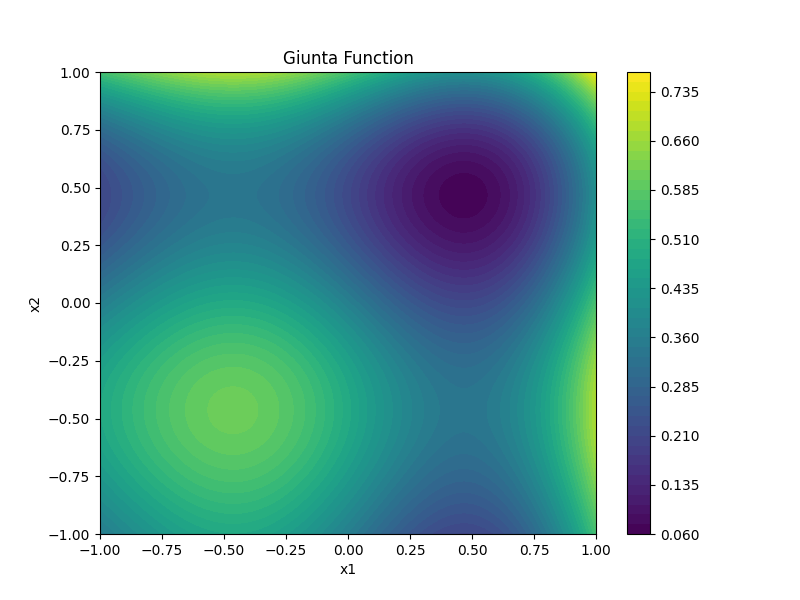
\includegraphics[width=0.8\textwidth]{images/giunta_function.png}
    \caption{Giunta Function.}
    \label{fig:giunta_function}
\end{figure}

Esta función presenta varias características que la 
hacen un reto interesante para los algoritmos de 
optimización:

\begin{itemize}
    \item \textbf{Continuidad:} La función es continua 
    en todo su dominio, lo que permite la aplicación 
    de una amplia gama de métodos de optimización.
    \item \textbf{Diferenciabilidad:} Es diferenciable, 
    lo que permite el uso de algoritmos que dependen 
    de la derivada, como los métodos de descenso de 
    gradiente.
    \item \textbf{Separabilidad:} La función puede 
    descomponerse en sumas de funciones más simples, 
    lo que podría simplificar la optimización en 
    ciertas circunstancias.
    \item \textbf{Escalabilidad:} Aunque en este 
    trabajo se estudia en un espacio de dos dimensiones, 
    la función puede generalizarse a dimensiones 
    superiores.
    \item \textbf{Multimodalidad:} La presencia de 
    múltiples óptimos locales hace que la búsqueda 
    del mínimo global sea un desafío, especialmente 
    para métodos que tienden a quedarse atrapados en 
    mínimos locales.
\end{itemize}

Dado que la función de Giunta es multimodal y presenta 
múltiples óptimos locales, es crucial elegir 
algoritmos que no solo sean capaces de encontrar un 
mínimo, sino que también tengan la capacidad de 
explorar adecuadamente el espacio de búsqueda para 
evitar caer en mínimos locales. En este estudio, 
se han seleccionado y probado los siguientes algoritmos:

\begin{itemize}
    \item \textbf{Métodos Clásicos:} Se han 
    implementado métodos como el 
    \textit{descenso máximo}, el \textit{método 
    cuasi-Newton (BFGS)}, y el \textit{método de 
    región de confianza}. Estos métodos son apropiados 
    para funciones diferenciables y proporcionan una 
    buena convergencia local.
    \item \textbf{Algoritmos Evolutivos:} Se incluye 
    la \textit{evolución diferencial} y el 
    \textit{algoritmo genético}, que son conocidos 
    por su capacidad para explorar grandes espacios 
    de búsqueda y su eficacia en la identificación 
    de óptimos globales.
    \item \textbf{Optimización Basada en Población:} 
    El \textit{algoritmo de enjambre de partículas 
    (PSO)} es otro enfoque utilizado, el cual es 
    efectivo en la búsqueda global, aprovechando la 
    cooperación entre partículas.
    \item \textbf{Algoritmos de Búsqueda Estocástica:} 
    Finalmente, se ha probado el \textit{recocido 
    simulado} y el \textit{método de salto de cuenca 
    (Basin Hopping)}, que son métodos robustos 
    frente a la multimodalidad, proporcionando una 
    exploración más extensa del espacio de búsqueda.
    \item \textbf{Función \texttt{minimize} de \texttt{scipy.optimize}:} 
    Esta función es un envoltorio general para la 
    optimización de minimización de funciones en 
    Python, que permite la aplicación de varios 
    algoritmos subyacentes como BFGS, L-BFGS-B, 
    SLSQP, entre otros. Es un enfoque flexible que 
    puede adaptarse a diferentes tipos de problemas 
    de optimización y ha sido incluido en este estudio 
    para comparar su rendimiento frente a otros 
    algoritmos especializados.
\end{itemize}

\subsection{Objetivo del Estudio}

El objetivo de este trabajo es evaluar la precisión y 
eficiencia de estos algoritmos al aproximarse al 
mínimo global de la función de Giunta. Se analizarán 
tanto los errores en la posición y el valor de la 
función respecto al óptimo global, como el tiempo 
computacional requerido para cada algoritmo.

Este análisis no solo proporcionará una comparación 
directa entre diferentes enfoques de optimización, 
sino que también permitirá identificar qué métodos 
son más adecuados para funciones multimodales como 
la de Giunta, en escenarios de optimización real.



\section{Algoritmos de Optimización}


\subsection{Descenso Máximo}

El método de \textit{descenso máximo}, también conocido como \textit{gradiente descendente}, es uno de los algoritmos de optimización más básicos y ampliamente utilizados. Este método se basa en la iteración hacia la dirección opuesta del gradiente de la función objetivo, con el objetivo de minimizarla.

\subsubsection{Aplicaciones y Efectividad}

El descenso máximo es especialmente efectivo en escenarios donde la función objetivo es convexa y diferenciable, ya que garantiza la convergencia hacia el mínimo global en tales casos. Es ampliamente utilizado en problemas de optimización continua y es la base para muchas variantes y métodos más sofisticados.

\subsubsection{Ventajas y Desventajas Generales}

\begin{itemize}
    \item \textbf{Ventajas:} 
    \begin{itemize}
        \item Simplicidad de implementación.
        \item Eficiencia en problemas convexos.
    \end{itemize}
    \item \textbf{Desventajas:} 
    \begin{itemize}
        \item Sensibilidad a la elección del tamaño de paso (learning rate).
        \item Propenso a quedar atrapado en óptimos locales en funciones no convexas.
    \end{itemize}
\end{itemize}

\subsubsection{Rendimiento en la Función de Giunta}

En la optimización de la función de Giunta, el método de descenso máximo presenta limitaciones significativas. Dado que la función es multimodal, este algoritmo tiende a quedar atrapado en los numerosos óptimos locales, lo que impide alcanzar el mínimo global. Además, la elección del tamaño de paso es crucial; un tamaño de paso inadecuado puede ralentizar la convergencia o causar que el algoritmo oscile sin converger.

\subsection{Método Cuasi-Newton (BFGS)}

El \textit{método cuasi-Newton}, y en particular el algoritmo BFGS (Broyden-Fletcher-Goldfarb-Shanno), es un método iterativo para encontrar el mínimo de una función diferenciable. Este método mejora el descenso máximo al utilizar una aproximación de la matriz Hessiana para ajustar el tamaño de paso y la dirección de búsqueda.

\subsubsection{Aplicaciones y Efectividad}

BFGS es ampliamente utilizado en problemas de optimización no lineal debido a su rapidez de convergencia y robustez, especialmente en funciones suaves y bien condicionadas. Es particularmente eficaz en escenarios donde se necesita un equilibrio entre la precisión y el costo computacional.

\subsubsection{Ventajas y Desventajas Generales}

\begin{itemize}
    \item \textbf{Ventajas:} 
    \begin{itemize}
        \item Convergencia más rápida que el descenso máximo.
        \item Menor dependencia en la elección del tamaño de paso.
    \end{itemize}
    \item \textbf{Desventajas:} 
    \begin{itemize}
        \item Mayor complejidad computacional debido a la estimación de la matriz Hessiana.
        \item Menor eficiencia en problemas de alta dimensionalidad o funciones mal condicionadas.
    \end{itemize}
\end{itemize}

\subsubsection{Rendimiento en la Función de Giunta}

En el caso de la función de Giunta, BFGS también enfrenta dificultades para evitar los óptimos locales debido a la multimodalidad de la función. No obstante, la capacidad de ajustar la dirección de búsqueda usando una aproximación de la matriz Hessiana permite una convergencia más eficiente hacia un óptimo local en comparación con el descenso máximo.

\subsection{Método de Región de Confianza}

El \textit{método de región de confianza} es un enfoque iterativo que ajusta el tamaño de la región en la que se confía que la aproximación cuadrática de la función es precisa. En cada iteración, se minimiza un modelo simplificado de la función dentro de esta región.

\subsubsection{Aplicaciones y Efectividad}

Este método es altamente efectivo en problemas donde la función objetivo es suavemente diferenciable y donde se requiere una robustez adicional frente a la posible mala condición de la matriz Hessiana. Es comúnmente utilizado en optimización no lineal y en aplicaciones que requieren una alta precisión en la convergencia.

\subsubsection{Ventajas y Desventajas Generales}

\begin{itemize}
    \item \textbf{Ventajas:} 
    \begin{itemize}
        \item Alta robustez frente a variaciones en la curvatura de la función.
        \item Ajuste dinámico de la región de búsqueda que mejora la convergencia.
    \end{itemize}
    \item \textbf{Desventajas:} 
    \begin{itemize}
        \item Complejidad computacional elevada.
        \item Puede ser ineficiente en problemas de alta dimensionalidad.
    \end{itemize}
\end{itemize}

\subsubsection{Rendimiento en la Función de Giunta}

Aunque el método de región de confianza es robusto en términos de convergencia, su aplicación en la función de Giunta está limitada por la multimodalidad de la función. Similar a otros métodos locales, este método puede quedar atrapado en óptimos locales, especialmente si la región de confianza es inicialmente grande y abarca múltiples picos de la función.

\subsection{Evolución Diferencial}

El \textit{algoritmo de evolución diferencial} es un método estocástico de optimización global que se basa en la mutación, cruce y selección para explorar el espacio de búsqueda. Es especialmente útil en problemas de optimización no convexos, discontinuos o multimodales.

\subsubsection{Aplicaciones y Efectividad}

Evolución diferencial es ampliamente utilizado en optimización global debido a su capacidad para explorar el espacio de búsqueda y evitar óptimos locales. Es eficaz en problemas donde otros métodos podrían fallar debido a la presencia de múltiples óptimos locales o superficies de respuesta irregulares.

\subsubsection{Ventajas y Desventajas Generales}

\begin{itemize}
    \item \textbf{Ventajas:} 
    \begin{itemize}
        \item Alta capacidad de exploración global.
        \item No requiere el cálculo de derivadas.
    \end{itemize}
    \item \textbf{Desventajas:} 
    \begin{itemize}
        \item Convergencia más lenta en comparación con métodos de optimización local.
        \item Depende de la elección de los parámetros de mutación y cruce.
    \end{itemize}
\end{itemize}

\subsubsection{Rendimiento en la Función de Giunta}

En la optimización de la función de Giunta, la evolución diferencial destaca por su capacidad para explorar el espacio de búsqueda y escapar de óptimos locales. Sin embargo, su convergencia puede ser más lenta que la de otros métodos locales, lo que puede ser una desventaja si se requiere una solución rápida.

\subsection{Algoritmo Genético}

El \textit{algoritmo genético} es un método de optimización inspirado en el proceso de selección natural. Utiliza operadores como la selección, cruce y mutación para evolucionar una población de soluciones y encontrar el óptimo global.

\subsubsection{Aplicaciones y Efectividad}

Los algoritmos genéticos son efectivos en problemas de optimización global, especialmente aquellos con múltiples óptimos locales, restricciones complejas o superficies de respuesta no suaves. Son aplicables en una variedad de dominios, desde el diseño de ingeniería hasta la inteligencia artificial.

\subsubsection{Ventajas y Desventajas Generales}

\begin{itemize}
    \item \textbf{Ventajas:} 
    \begin{itemize}
        \item Capacidad para escapar de óptimos locales.
        \item Flexibilidad para manejar problemas con restricciones no lineales y dominios discretos.
    \end{itemize}
    \item \textbf{Desventajas:} 
    \begin{itemize}
        \item Convergencia relativamente lenta.
        \item Dependencia en la configuración de parámetros como la tasa de mutación y cruce.
    \end{itemize}
\end{itemize}

\subsubsection{Rendimiento en la Función de Giunta}

Para la función de Giunta, los algoritmos genéticos son altamente efectivos para evitar los óptimos locales, dada la multimodalidad de la función. No obstante, similar a la evolución diferencial, la convergencia puede ser lenta y depende de una buena configuración de los parámetros del algoritmo.

\subsection{Algoritmo de Enjambre de Partículas (PSO)}

El \textit{algoritmo de enjambre de partículas (PSO)} es un método de optimización que simula el comportamiento de un grupo de partículas en movimiento dentro del espacio de búsqueda. Las partículas ajustan su posición en función de su experiencia personal y la del enjambre, buscando el óptimo global.

\subsubsection{Aplicaciones y Efectividad}

PSO es adecuado para problemas de optimización global, especialmente aquellos con múltiples óptimos locales. Es comúnmente utilizado en problemas de alta dimensionalidad y en aplicaciones donde se requiere una búsqueda global efectiva.

\subsubsection{Ventajas y Desventajas Generales}

\begin{itemize}
    \item \textbf{Ventajas:} 
    \begin{itemize}
        \item Buena capacidad para encontrar el óptimo global.
        \item Menor dependencia en la elección de parámetros en comparación con algoritmos genéticos.
    \end{itemize}
    \item \textbf{Desventajas:} 
    \begin{itemize}
        \item Posibilidad de convergencia prematura.
        \item Sensibilidad a la elección de ciertos parámetros como el coeficiente de inercia.
    \end{itemize}
\end{itemize}

\subsubsection{Rendimiento en la Función de Giunta}

En la función de Giunta, PSO se muestra como un método eficaz para evitar los óptimos locales y encontrar el mínimo global. Sin embargo, existe el riesgo de convergencia prematura si las partículas se agrupan demasiado rápido en una región subóptima del espacio de búsqueda.

\subsection{Recocido Simulado}

El \textit{recocido simulado} es un algoritmo estocástico de optimización global inspirado en el proceso de recocido en metalurgia. El algoritmo permite que el sistema explore soluciones subóptimas en etapas tempranas, reduciendo gradualmente la probabilidad de aceptar soluciones peores a medida que avanza la búsqueda.

\subsubsection{Aplicaciones y Efectividad}

Recocido simulado es útil en problemas de optimización global, especialmente aquellos con superficies de búsqueda complejas y múltiples óptimos locales. Es eficaz para evitar quedar atrapado en mínimos locales, aunque puede requerir un tiempo considerable para alcanzar la convergencia.

\subsubsection{Ventajas y Desventajas Generales}

\begin{itemize}
    \item \textbf{Ventajas:} 
    \begin{itemize}
        \item Capacidad para escapar de mínimos locales.
        \item No requiere el cálculo de derivadas, siendo útil en funciones no diferenciables.
    \end{itemize}
    \item \textbf{Desventajas:} 
    \begin{itemize}
        \item Convergencia lenta.
        \item Sensibilidad a la elección de la programación de enfriamiento.
    \end{itemize}
\end{itemize}

\subsubsection{Rendimiento en la Función de Giunta}

Para la función de Giunta, el recocido simulado es un enfoque robusto que puede evitar los óptimos locales, pero su lenta convergencia puede ser una desventaja en escenarios donde el tiempo computacional es un factor crítico.

\subsection{Método de Salto de Cuenca (Basin Hopping)}

El \textit{método de salto de cuenca} es un enfoque de optimización global que combina la búsqueda local con saltos aleatorios entre diferentes regiones del espacio de búsqueda. Este método es particularmente útil para funciones multimodales.

\subsubsection{Aplicaciones y Efectividad}

Basin Hopping es efectivo en problemas donde la función objetivo tiene múltiples mínimos locales. Es comúnmente utilizado en química computacional y biología estructural para encontrar las configuraciones energéticas más bajas.

\subsubsection{Ventajas y Desventajas Generales}

\begin{itemize}
    \item \textbf{Ventajas:} 
    \begin{itemize}
        \item Capacidad para explorar múltiples cuencas de atracción.
        \item Combinación efectiva de búsqueda local y global.
    \end{itemize}
    \item \textbf{Desventajas:} 
    \begin{itemize}
        \item Puede requerir ajustes finos en los parámetros de salto.
        \item La eficiencia depende del éxito del método local utilizado en cada cuenca.
    \end{itemize}
\end{itemize}

\subsubsection{Rendimiento en la Función de Giunta}

En la función de Giunta, Basin Hopping muestra un rendimiento notable, ya que su combinación de saltos globales y búsqueda local permite evitar los óptimos locales. No obstante, la elección del método local puede influir significativamente en la efectividad del algoritmo.

\subsection{Función \texttt{minimize} de \texttt{scipy.optimize}}

La función \texttt{minimize} de \texttt{scipy.optimize} es un envoltorio que permite aplicar varios algoritmos de minimización a funciones continuas. Los métodos disponibles incluyen BFGS, L-BFGS-B, SLSQP, entre otros.

\subsubsection{Aplicaciones y Efectividad}

La función \texttt{minimize} es útil en una amplia gama de problemas de optimización debido a su flexibilidad y facilidad de uso. Es particularmente efectiva en funciones suavemente diferenciables donde se necesita una solución rápida y eficiente.

\subsubsection{Ventajas y Desventajas Generales}

\begin{itemize}
    \item \textbf{Ventajas:} 
    \begin{itemize}
        \item Flexibilidad para seleccionar el método de optimización más adecuado.
        \item Fácil de implementar y ajustar.
    \end{itemize}
    \item \textbf{Desventajas:} 
    \begin{itemize}
        \item Limitada en su capacidad para manejar funciones altamente multimodales sin modificaciones.
        \item La efectividad depende del método específico seleccionado dentro de la función.
    \end{itemize}
\end{itemize}

\subsubsection{Rendimiento en la Función de Giunta}

En la función de Giunta, el rendimiento de \texttt{minimize} depende en gran medida del método subyacente seleccionado. Si bien los métodos como BFGS pueden ser rápidos y eficientes para encontrar óptimos locales, la función es propensa a quedarse atrapada en estos mínimos debido a la multimodalidad de la función de Giunta.

\subsection{Inaplicabilidad del Algoritmo de Newton}

El \textit{algoritmo de Newton} es un método de optimización que utiliza la matriz Hessiana completa para ajustar la dirección y el tamaño de los pasos en la búsqueda del mínimo de una función. Aunque es un método muy eficaz para problemas convexos y bien condicionados, presenta limitaciones significativas cuando se aplica a funciones no lineales y multimodales como la función de Giunta.

\subsubsection{Limitaciones en la Función de Giunta}

La función de Giunta es altamente no lineal y presenta una estructura multimodal con múltiples mínimos locales. El algoritmo de Newton, al ser un método de optimización local, asume que la función objetivo puede ser bien aproximada por una parábola en torno a un punto de interés, lo cual es efectivo en funciones suaves y convexas. Sin embargo, debido a la complejidad y no linealidad de la función de Giunta, esta suposición falla, lo que puede llevar a resultados imprecisos o a una convergencia hacia óptimos locales no deseados.

Además, la no linealidad de la función de Giunta implica que la matriz Hessiana puede ser extremadamente difícil de calcular y manejar, ya que puede estar mal condicionada o variar drásticamente en diferentes regiones del espacio de búsqueda. Esto no solo incrementa el costo computacional del algoritmo, sino que también puede resultar en direcciones de descenso ineficaces, haciendo que el método sea poco fiable y susceptible a quedarse atrapado en mínimos locales.

Por estas razones, se ha decidido no implementar el algoritmo de Newton en el presente estudio, dado que los métodos seleccionados ofrecen una mejor capacidad para lidiar con las características no lineales y multimodales de la función de Giunta.




\section{Resultados}
\subsection{Precisión en la Solución}

La precisión de los algoritmos se evaluó en términos 
del error en la posición \( \mathbf{x} \) encontrada 
en comparación con el mínimo global conocido 
\( \mathbf{x}^* \), así como el valor de la función 
\( f(\mathbf{x}) \) en ese punto. La Figura 
\ref{fig:error_in_position} muestra los errores en 
la posición para cada uno de los algoritmos, mientras 
que la Tabla \ref{tab:optimization_results} resume los 
valores obtenidos.

\begin{figure}[h!]
    \centering
    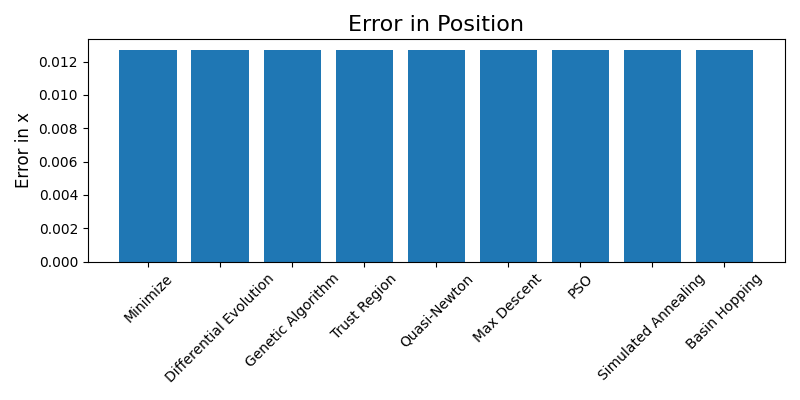
\includegraphics[width=0.8\textwidth]{images/error_in_position.png}
    \caption{Error en la posición obtenida por cada algoritmo.}
    \label{fig:error_in_position}
\end{figure}

Véase como los algoritmos mostraron rendimientos similares
y relativamente buenos en la aproximación del mínimo global de la Giunta Function.

\subsection{Tiempo Computacional}

El tiempo computacional requerido por cada uno de los 
algoritmos para converger a una solución se muestra en 
la Figura \ref{fig:time_taken}. Es notable que algunos 
algoritmos como Genetic Algorithm, Simulated Annealing, 
y Basin Hopping requieren significativamente más 
tiempo en comparación con métodos como Minimize o 
Quasi-Newton.

\begin{figure}[h!]
    \centering
    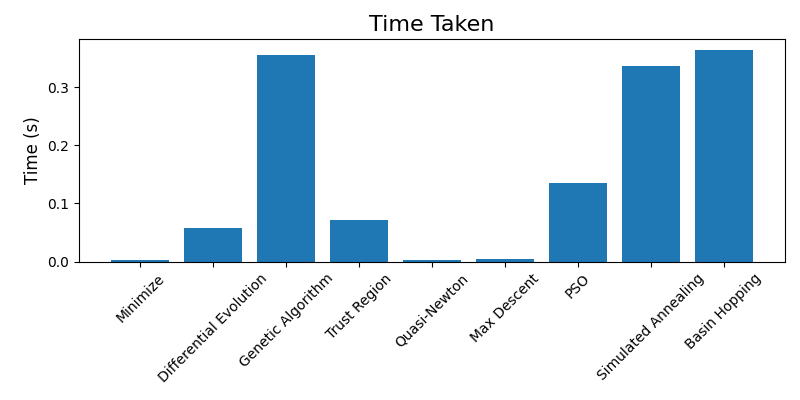
\includegraphics[width=0.8\textwidth]{images/time_taken.png}
    \caption{Tiempo de ejecución de cada algoritmo.}
    \label{fig:time_taken}
\end{figure}

\subsection{Resumen de Resultados}

Los resultados específicos de cada algoritmo se 
presentan en la Tabla \ref{tab:optimization_results}. 
Los valores de \( \mathbf{x} \) obtenidos se 
redondearon a 8 lugares decimales para asegurar una 
comparación clara y concisa. Esta tabla permite 
observar las diferencias en precisión y tiempo de 
manera más detallada.\\

\begin{table}[h!]
    \centering
    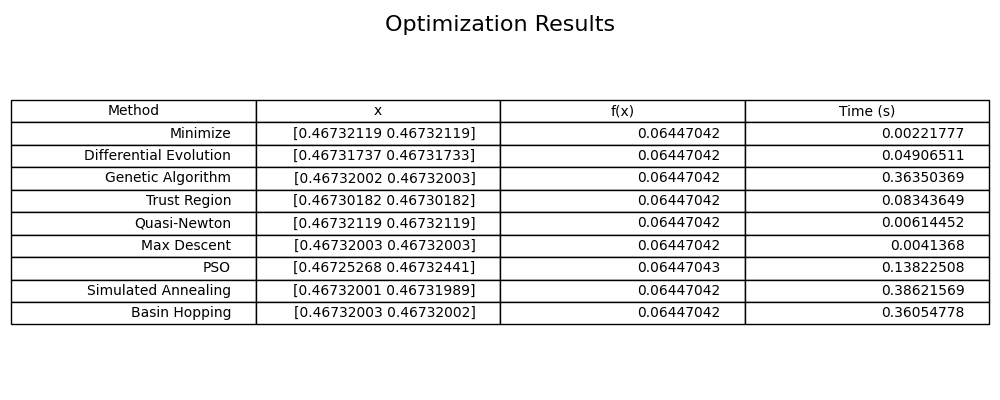
\includegraphics[width=0.8\textwidth]{images/optimization_results.png}
    \caption{Resumen de los resultados de optimización.}
    \label{tab:optimization_results}
\end{table}

También en la tabla \ref{tab:errors_relative_table} 
podemos apreciar detalladamente los errores a la hora 
de encontrar el punto de mínimo y en la evaluación de 
la función. Como ilustraba la figura 
\ref{fig:error_in_position}, los algoritmos alcanzaron 
soluciones significativamente similares.

\begin{table}[h!]
    \centering
    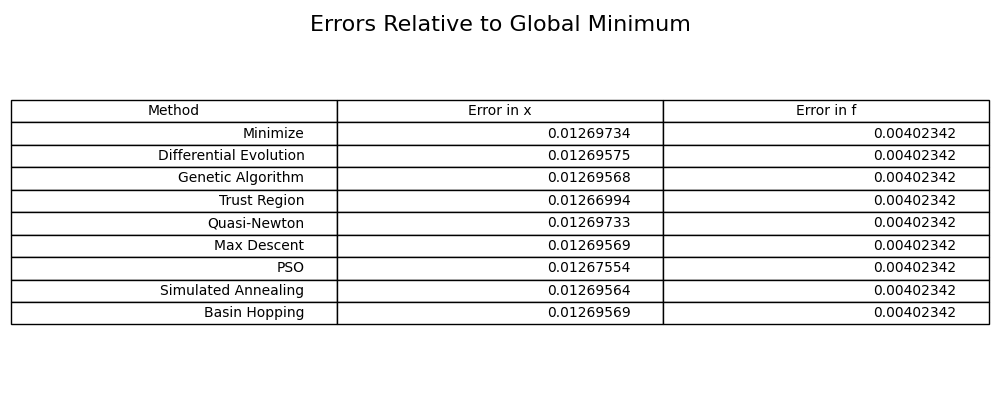
\includegraphics[width=0.8\textwidth]{images/errors_relative_table.png}
    \caption{Errores relativos al mínimo global.}
    \label{tab:errors_relative_table}
\end{table}

\subsection{Observaciones sobre el Comportamiento con Dimensiones Crecientes}

El análisis del comportamiento de los algoritmos de optimización con dimensiones 
crecientes es crucial, dado que muchos problemas en la práctica no se limitan a 
espacios de baja dimensionalidad. En este contexto, se deben considerar varios 
factores que afectan el rendimiento de los algoritmos estudiados cuando se 
incrementa la dimensionalidad del problema, en este caso, la Giunta Function.

\begin{itemize}
    \item \textbf{Métodos Clásicos:}
    Los métodos como el \textit{descenso máximo}, \textit{quasi-Newton} (BFGS), y el \textit{método de región de confianza} tienden a enfrentar desafíos significativos en espacios de alta dimensionalidad. La principal dificultad radica en la complejidad computacional que aumenta con el número de dimensiones, especialmente para BFGS, donde la necesidad de calcular y almacenar la matriz Hessiana aproximada se vuelve prohibitiva. Además, estos métodos son propensos a quedar atrapados en mínimos locales, un problema que se acentúa a medida que aumenta la cantidad de dimensiones y, por lo tanto, el número de óptimos locales. Esto implica que, aunque estos algoritmos pueden ser eficientes en espacios de baja a mediana dimensionalidad, su aplicabilidad disminuye en problemas de alta dimensionalidad.
    \item \textbf{Algoritmos Evolutivos y Basados en Población:}
    Los algoritmos evolutivos, como la \textit{evolución diferencial} y los \textit{algoritmos genéticos}, así como el \textit{algoritmo de enjambre de partículas} (PSO), son más adecuados para manejar el incremento dimensional debido a su capacidad intrínseca para explorar grandes espacios de búsqueda. Estos métodos tienden a mantener una buena capacidad exploratoria incluso en espacios de alta dimensionalidad, lo que les permite evitar quedarse atrapados en óptimos locales. Sin embargo, esto viene a costa de un aumento significativo en el tiempo computacional, ya que la evaluación de las funciones objetivo en un espacio de mayor dimensión es inherentemente más costosa.
    \item \textbf{Métodos Estocásticos:}
    El \textit{recocido simulado} y el \textit{salto de cuenca} (Basin Hopping) también son robustos frente al incremento dimensional, principalmente debido a su capacidad para realizar exploraciones globales del espacio de búsqueda. No obstante, su rendimiento en términos de tiempo puede ser considerablemente afectado, ya que la exploración estocástica de un espacio de búsqueda más grande generalmente requiere más iteraciones para alcanzar la convergencia. Además, la eficacia de estos métodos puede depender fuertemente de la parametrización del algoritmo, la cual puede necesitar ajustes más finos en espacios de alta dimensionalidad.
    
\end{itemize}

La selección del algoritmo de optimización más adecuado para problemas de alta dimensionalidad debe balancear la necesidad de precisión y la capacidad de evitar óptimos locales con el costo computacional. Algoritmos como la evolución diferencial, PSO, y recocido simulado son generalmente preferibles en escenarios de alta dimensionalidad, a pesar de sus mayores requisitos computacionales, mientras que los métodos clásicos pueden verse limitados por la complejidad computacional y su tendencia a converger en mínimos locales.



\section{Conclusiones}

El presente estudio ha proporcionado un análisis exhaustivo del rendimiento de diversos algoritmos de optimización aplicados a la Giunta Function, una función multimodal que presenta desafíos significativos debido a la presencia de múltiples óptimos locales. Se evaluaron tanto algoritmos clásicos como avanzados, considerando su precisión para aproximarse al mínimo global y el tiempo computacional requerido para alcanzar dicha solución. 

Los resultados obtenidos permiten extraer varias conclusiones clave:

\begin{itemize}
    \item \textbf{Precisión y Convergencia:} Los métodos clásicos, como el \textit{descenso máximo} y \textit{quasi-Newton} (BFGS), demostraron una buena capacidad de convergencia en escenarios de baja dimensionalidad, sin embargo, su propensión a quedarse atrapados en óptimos locales limita su aplicabilidad en funciones multimodales como la Giunta Function. Estos métodos son más adecuados cuando se busca una solución rápida en un entorno donde la función objetivo es suave y diferenciable, pero son menos efectivos en la búsqueda global.

    \item \textbf{Exploración Global:} Los algoritmos evolutivos, como la \textit{evolución diferencial} y los \textit{algoritmos genéticos}, junto con el \textit{algoritmo de enjambre de partículas} (PSO), mostraron una mayor capacidad para evitar quedar atrapados en óptimos locales, logrando una exploración más efectiva del espacio de búsqueda. Aunque estos algoritmos requieren un mayor tiempo computacional, son preferibles en problemas multimodales o de alta dimensionalidad, donde la exploración global es crucial.

    \item \textbf{Robustez en Dimensiones Crecientes:} Al aumentar la dimensionalidad del problema, los métodos estocásticos como el \textit{recocido simulado} y el \textit{salto de cuenca} (Basin Hopping) demostraron una robustez significativa. Estos métodos, aunque más lentos en convergencia, son capaces de explorar de manera efectiva grandes espacios de búsqueda y evitar la convergencia prematura en mínimos locales. Su capacidad para ajustar dinámicamente la búsqueda en función de la topología del espacio de búsqueda los hace especialmente útiles en problemas complejos y de alta dimensionalidad.

    \item \textbf{Tiempo Computacional:} Un aspecto crucial en la selección del algoritmo adecuado es el balance entre la precisión y el tiempo computacional. Los métodos como \textit{BFGS} y el \textit{método de región de confianza} son rápidos en su convergencia hacia un óptimo local, pero este beneficio se ve contrarrestado por su susceptibilidad a quedar atrapados en óptimos locales. Por otro lado, aunque los algoritmos evolutivos y estocásticos requieren más tiempo, ofrecen una mejor exploración global y son más fiables en problemas de mayor complejidad.

\end{itemize}

En resumen, la elección del algoritmo de optimización debe basarse en las características específicas del problema a resolver. Para funciones multimodales y problemas de alta dimensionalidad, los métodos estocásticos y evolutivos son generalmente más efectivos, a pesar de su mayor costo computacional. Los métodos clásicos, aunque rápidos y eficientes en escenarios más simples, deben usarse con precaución cuando se enfrentan a problemas con una topología compleja, como la Giunta Function. Este estudio proporciona una guía valiosa para seleccionar el método más apropiado en función de las características del problema y las limitaciones de tiempo computacional.

\end{document}
